\documentclass[14pt]{extarticle}



%other%
\usepackage[russian]{babel}
\usepackage{polyglossia}
\usepackage{graphicx}
\usepackage{float}
%other%


%math%
\usepackage{amsthm}
\usepackage{amsmath}
\usepackage{amssymb}
\usepackage{unicode-math}
\newtheorem*{lemma}{\textup{Задача}}
\newtheorem*{corollary}{\textup{Комментарий}}

\renewcommand\qedsymbol{$\blacksquare$}

%math%

%page geometry%
\usepackage[margin=0.7in]{geometry}


%page geometry%

%fonts%
\setdefaultlanguage[spelling=modern]{russian}
\setotherlanguage{english}
\setmainfont{CMU Serif}
\setsansfont{CMU Sans Serif}
\setmonofont{CMU Typewriter Text}  
\setmathfont{Latin Modern Math}
%fonts%


\newenvironment{rcases}
  {\left.\begin{aligned}}
  {\end{aligned}\right\rbrace}


\begin{document}

\begin{lemma}
	\textup{
	Окружности $\omega_1$ и $\omega_2$ пересекаются
	в точках $A$ и $B$. В точке $A$ к окружностям $\omega_1$
	и $\omega_2$ соответственно
	построены касательные $l$ и $k$, пересекающие окружности
	соответственно в точках $D$ и $C$.
	Докажите, что $AC^2 \cdot BD = AD^2 \cdot BC$.
    }
\end{lemma}

\begin{proof}[\bf{\textup{Решение}}]
	
	\begin{figure}[H]
	\centering
	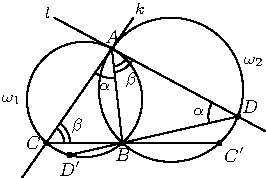
\includegraphics[width=8cm]{./img/img.pdf}
    \end{figure}
    

    Пусть $\angle BAC = \alpha$, а $\angle BAD = \beta$. 
	Тогда $\angle BDA = \alpha$ по теореме об угле между
	хордой и касательной. Аналогично $\angle BCA = \beta$.
	Из подобия $ \bigtriangleup ABC \sim  \bigtriangleup DBA $
	следует, что $\frac{AC}{AD} = \frac{BC}{BA} = \frac{BA}{BD}$.
	Отсюда сразу следует, что $\frac{AC^2}{AD^2} = 
	\frac{BC}{BA} \cdot \frac{BA}{BD} = \frac{BC}{BD}$
	Домножая обе части полученного равенства ($\frac{AC^2}{AD^2} = 
	\frac{BC}{BD}$) на $\frac{AD^2}{BD}$ (метод креста)
	получим требуемое утверждение: $AC^2 \cdot BD = AD^2 \cdot BC$.
\end{proof}

\begin{corollary}
	\textup{
	Несложно видеть интересный факт, как следствие доказаной задачи,
	a именно $DD' = CC'$. Это верно в силу того что 
	$deg(C, \omega_2) = AC^2 = CB \cdot CC'$, а также 
    $deg(D, \omega_1) = AD^2 = DB \cdot DD'$. 
    }   

	%\begin{equation*}
	%	\begin{cases}
	%	$AC^2 &= BC$
		%AC^2 \cdot BD & AD^2 \cdot BC \\
		%AC^2 &= CB \cdot CC' \\
		%AD^2 &= DB \cdot DD'
       % \end{cases}
	%\end{equation*}

	
\begin{equation*}
\begin{rcases}
	AC^2 \cdot BD &= AD^2 \cdot BC\\
	AC^2 &= BC \cdot CC'\\
    AD^2 &= BD \cdot DD'
\end{rcases} 
\text{$\Rightarrow DD' = CC'$}
\end{equation*} 	
	    %\text{$AC^2 \cdot BD = AD^2 \cdot BC$}\\
	   %\text{$AC^2 = CB \cdot CC'$}\\
	   %\text{$AD^2 = DB \cdot DD'$}\\ 
    
\end{corollary}


\end{document}
